\documentclass[10pt]{book}
\usepackage[utf8]{inputenc}
\usepackage[italian]{babel}
\usepackage{multicol}
\usepackage[bookmarks]{hyperref}
\usepackage[a4paper, total={18cm, 25cm}]{geometry}
\usepackage{listings}
\usepackage{graphicx}
\usepackage{makecell}
\graphicspath{ {./img/} }
\usepackage{color}

\begin{document}
\renewcommand*\contentsname{Indice}
\title{Crittografia}
\author{Federico Matteoni}
\date{A.A. 2020/21}
\maketitle
\tableofcontents
\pagebreak
\section*{Introduzione}
Prof.ssa: Anna Bernasconi.\\
Vedremo i cifrari da un punto di vista prettamente algoritmico. Vedremo anche i cifrari storici, ormai non più utilizzabili, perché hanno "aperto la strada", per poi passare ai cifrari perfetti (soluzione ideale ma con costo elevato).\\
Poi esamineremo i cifrari simmetrici, a chiave pubblica, curve ellittiche, firma digitale, SSL. Protocolli zero knowledge, blockchain e crittografia quantistica.\\\\
Libro di testo: Bernasconi, Ferragina, Luccio - Elementi di Crittografia.
\paragraph{Esame} Orali nel caso di esami a distanza, scritto nel caso di esami in presenza, closed-book.
\chapter{Introduzione alla Crittografia}
\section{Introduzione}
\paragraph{Crittografia} Significa "\textit{scrittura nascosta}", si intendono tecniche matematiche per mascherare i messaggi per non renderli leggibili a terzi (\textbf{crittografia}) o tentare di svelarli quando non si è il legittimo destinatario (\textbf{crittoanalisi}). Quindi tecniche di protezione e viceversa.\\
Esiste per i due mondi in contrapposizione: persone che vogliono scambiarsi privatamente informazioni e gli \textit{impiccioni} che desiderano ascoltare o intromettersi nelle conversazioni altrui (per curiosità, investigazione o altri scopi).
\paragraph{Due gruppi di persone} Chi vuole proteggersi userà \textbf{metodi di cifratura}, gli altri useranno \textbf{metodi di crittoanalisi}
\subparagraph{Crittografia} Metodi di Cifratura
\subparagraph{Crittoanalisi} Metodi di \ldots
\textbf{crittologia} studio comunicazione canali non sicuri e relativi problemi
\subsection{Lo scenario}
Alice vuole comunicare con Bob su un canale insicuro, quindi adottano un metodo di cifratura per spedire il messaggio in chiaro \texttt{m} sottoforma di crittogramma \texttt{c} (testo cifrato) che deve essere: incomprensibile al crittoanalista Eve (eavesdropper) in ascolto sul canale, ma facilmente decifrabile da Bob.
\paragraph{MSG} Insieme dei messaggi in chiaro
\paragraph{CRITTO} Insieme dei crittogrammi
\begin{center}
C : MSG $\rightarrow$ CRITTO\\
D : CRITTO $\rightarrow$ MSG
\end{center}
Sono operazioni da poter fare in tempo polinomiale. 
C e D sono una l'inversa dell'altra, ma C \textbf{deve essere iniettiva}.
\begin{center}
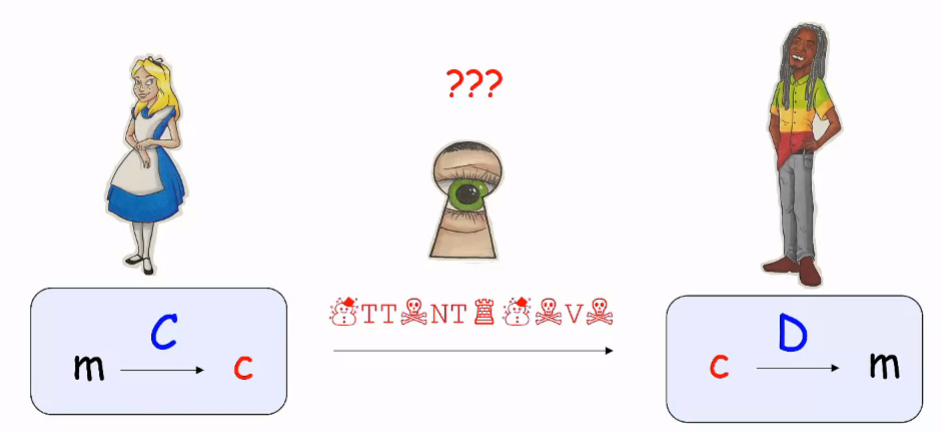
\includegraphics[scale=0.55]{1.png}
\end{center}
\subsection{Antichi esempi}
\paragraph{Erodoto} Nelle \textit{Storie}, V secolo a.C.\\
Messaggi tatuati sulla testa, coperti dai capelli e riscoperti rasando la testa.
\paragraph{Scitale} Spartani. Asta cilindrica in due esemplari identici. Si avvolgeva una striscia di carta attorno al cilindro e scritta. La chiave del cifrario è il diametro dello scitale.
\begin{center}
	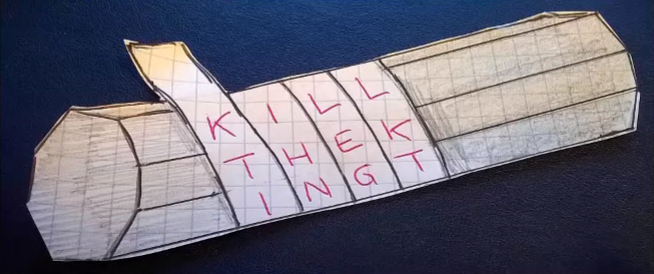
\includegraphics[scale=0.5]{2.png}
\end{center}
\paragraph{Enea Tattico} Un libro qualsiasi con un insieme di lettere segnate, o sostituire le vocali con simboli grafici.
\paragraph{Cifrario di Cesare} Il più antico cifrario di concezione moderna. L'idea di base è che il crittogramma è ottenuto dal messaggio in chiaro \texttt{m} sostituendo ogni lettera con quella di tre posizioni più avanti nell'alfabeto.\\
Es. A $\rightarrow$ D, Z $\rightarrow$ C. La segretezza dipende interamente dalla conoscenza del metodo, era destinato all'uso ristretto da un piccolo gruppo di persone.
\section{Livello di segretezza}
\paragraph{Classificazione} in base al livello di segretezza
\begin{list}{}{}
	\item Cifrari per \textbf{uso ristretto}\\
	Le tecniche con cui si calcola e decifra il crittogramma sono tenute segrete in ogni loro aspetto. Impiegati per comunicazioni classificate (diplomatiche o militari), non adatti per uso di massa.
	\item Cifrari per \textbf{uso generale}\\
	Ogni codice segreto non può essere mantenuto tale per troppo a lungo. La parte segreta si limita alla chiave, nota solamente agli utenti che stanno comunicando.\\
	Vengono studiati dalla comunità, coinvolgendo tantissime persone. Solo la chiave deve essere segreta.\\
	\textbf{Il nemico conosce il sistema}.\\
	Quindi C e D sono note, la chiave \textbf{segreta}\texttt{k} è usata come input sia in C che in D:\\
	\texttt{c = C(m, k)}, \texttt{m = D(c, k)}\\
	Se non si conosce \texttt{k}, anche conoscendo C e D non si possono estrarre informazioni dal crittogramma.\\
	Tenere segreta una sola chiave è più facile che segretare l'intero metodo. Tutti possono usare C e D pubbliche con chiavi diverse, e se un crittoanalista entra in possesso di una chiave posso generarne semplicemente una nuova.
\end{list}
\subsection{Chiavi segreta} Se la segretezza dipende unicamente dalla chiave bisogna proteggersi dagli attacchi a forza bruta, quindi avere un gran numero di chiavi, così da essere immuni da chi le prova tutte.\\
Inoltre la chiave deve essere scelta in modo casuale e non prevedibile, sennò il crittoanalista può provare le chiavi ovvie.
\paragraph{Attacco esauriente} Il crittoanalisa potrebbe sferrare un attacco a forza bruta verificando la significatività delle sequenze \texttt{D(c, k)} $\forall$ \texttt{k}.\\
Se $|$Key$|$ = $10^{20}$ e con un calcolatore che impiega $10^{-6}$ per calcolare \texttt{D(c, k)} servirebbe in media più di un milione di anni per scoprire il messaggi provando tutte le chiavi. Però la segretezza può essere violata con altre tecniche: esistono cifrari più sicuri di altri pur con uno spazio di chiavi più piccoli.\\
Un cifrario complicato non è necessariamente più sicuro e \textbf{mai sottovalutare la bravura del crittoanalista}.
\subsection{Crittoanalista}
%TODO
\paragraph{Attacchi a un sistema crittografico} Hanno l'obiettivo di forzare un sistema. Il metodo e il livello di pericolosità dipendono dalle informazioni in possesso del crittoanalista:
\begin{list}{}{}
	\item Cipher Text Attack: conosce una serie di crittogrammi
	\item Known Plain-Text Attack: conosce una serie di coppie \texttt{(m, c)}
	\item Chosen Plain-Text Attack: si procura coppie \texttt{(m, c)} relative a messaggi in chiaro da lui scelti. Tutta la crittografia a chiave pubblica è soggetta.
\end{list}
\paragraph{Man in the Middle}
\paragraph{Esiti}
\begin{list}{}{}
	\item Successo pieno, si scopre completamente D o si ottiene la chiave
	\item Successo limitato, si scopre solo qualche informazione ma sufficiente per comprendere il messaggio
\end{list}
\subsection{Situazione attuale}
\paragraph{Cifrari perfetti} Inattaccabili, esistono ma richiedono operazioni complesse e chiavi lunghe tanto quanto il messaggio e mai riusabili.\\
\textbf{Shannon}, 1945 (pubblicato nel 1949 per motivi di segretezza militare): \texttt{m} e \texttt{c} appaiono totalmente scorrelati, come se \texttt{c} fosse una stringa casuale di bit.\\Nessuna informazione può filtrare dal crittogramma. Vedremo la teoria matematica.
\subparagraph{One-Time Pad} Anche detto blocco monouso, sicuro ma per essere usato bene richiede chiavi segrete totalmente casuali e lunghe quanto il messaggio. Come generarla e come scambiarla?
\paragraph{Cifrari attuali} Nella crittografia di massa non si usano cifrari perfetti, ma cifrari \textbf{dichiarati} sicuri, inviolati dagli esperti e che usano algoritmi solo esponenziali per decrittare senza chiave. Il tempo per violare un cifrario è enorme e rende l'operazione insostenibile $\rightarrow$ impossibilità \textit{pratica} di forzare il cifrario.
\subparagraph{Dichiarati sicuri} Non è noto se questi problemi matematici richiedano algoritmi \textit{necessariamente} esponenziali o se sono dovuti all'incapacità nostra di trovare metodi più efficienti. Si riconduce a $P ? NP$
\subsection{Cifrari odierni}
\paragraph{Advanced Encryption Standard} AES, simmetrico a blocchi con chiavi di 128-256bit, pubblicamente noto e realizzabile su computer di ogni tipo. Il messaggio è diviso a blocchi lunghi quanto la chiave.
\paragraph{Le chiavi} Sono stabilite dai mezzi elettronici (PC, smartphone, terminale...) e su Internet si scambia una chiave per ogni sessione.
\subparagraph{Scambio delle chiavi} La chiave va comunicata in sicurezza su un canale non ancora sicuro. Un'intercettazione nello scambio della chiave compromette il sistema.\\
Nel 1976 viene proposto un algoritmo per generare e scambiare una chiave segreta su un canale insicuro, senza necessità di scambiare informazioni o di incontrarsi in precedenza.\\
Si chiama \textbf{protocollo DH}, ancora largamente utilizzato nei protocolli crittografici su Internet.\\
Si scambiano pezzi di chiave tramite la rete e unendole a informazioni locali si costruisce la chiave.
\subparagraph{Chiave pubblica} Diffie ed Hellman hanno anche proposto la crittografia a chiave pubblica.
\begin{list}{}{}
	\item \textbf{Cifrari simmetrici}: stessa chiave per cifrare e decifrare, nota solo ai due utenti che comunicano. La scelgono di comune accordo e la tengono segreta.
	\item \textbf{Cifrari asimmetrici}: chiavi pubbliche usate per cifrare e chiavi private per decifrare.\\
	\texttt{c = C(m, k$_{pub}$)}\\
	\texttt{m = D(m, k$_{prv}$)}\\
	Si rende necessario che la C sia una one-way trapdoor: calcolare il crittogramma deve essere facile (polinomiale), ma decifrare \texttt{c} deve essere computazionalmente difficile (a meno di conoscere la trapdoor, la chiave privata).
\end{list}
\paragraph{RSA} Rivest, Shamir, Adleman, 1977. Propongono un sistema a chiave pubblico facile da calcolare e difficile da invertire.
\paragraph{Vantaggi}
\begin{list}{}{}
	\item Comunicazione molti a uno\\
	Tutti possono inviare in modo sicuro allo stesso destinatario usando la sua chiave pubblica, ma solo lui può decifrarli. Un crittoanalista non può decifrare anche se conosce C, D e k$_{pub}$
	\item Se $n$ utenti vogliono comunicare servono solo $2n$ chiavi invece delle $n(n-1)/2$ necessarie nei cifrari simmetrici (una coppia per ogni coppia di utenti)
	\item Non è richiesto nessun scambio
\end{list}
\paragraph{Svantaggi}
\begin{list}{}{}
	\item Sono molto lenti rispetto ai cifrari simmetrici (polinomi di terzo grado)
	\item Sono esposti ad attacchi di tipo chosen plain-text, perché conosco la chiave pubblica\\
	Scelgo un numero qualsiasi di messaggi in chiaro, costruisce i crittogrammi relativi e ascolta sul canale confrontando i crittogrammi in transito e se trova un riscontro sa esattamente qual è il messaggio passato.
\end{list}
\paragraph{Come si usa} Oggi si usa un cifrario a chiave segreta (AES) per le comunicazioni di massa, e un cifrario a chiave pubblica per scambiare le chiavi segrete relative al primo senza incontri fisici tra gli utenti.\\
Diventa lento solo lo scambio delle chiavi. Siamo anche al sicuro da attacchi chosen plain-text perché se la chiave è scelta bene risulta imprevedibile dal crittoanalista.
\section{Rappresentazione matematica di oggetti}
Per rappresentare gli oggetti scegliamo dei \textbf{caratteri} da un \textbf{insieme finito} detto \textbf{alfabeto}.\\
Un \textbf{oggetto} è \textbf{rappresentato da una sequenza ordinata di caratteri dell'alfabeto}. L'ordine dei caratteri è importante: a \textbf{oggetti diversi corrispondono sequenze diverse} e \textbf{il numero di oggetti che si possono rappresentare non ha limiti}. Significa che fissando un numero $n$ arbitrariamente grande possiamo sempre creare un numero di oggetti $> n$, con sequenze via via più grande.
\paragraph{Alfabeto} $\Gamma$ con $|\Gamma| = s$ e $N$ oggetti da rappresentare.\\
$d(s, N)$: lunghezza della sequenza più lunga che rappresenta un oggetto dell'insieme. A noi interessa la rappresentazione che minimizza $d(s, N)$, cioè $d_{min}(s, N)$\\
Una rappresentazione è tanto più efficiente quanto $d(s, N)$ si avvicina a $d_{min}(s, N)$
\paragraph{Esempio} $s = 1, \Gamma = \{0\}$ l'unica possibilità è variare la lunghezza $\Rightarrow d_{min}(1, N) = N$, estremamente sfavorevole.\\
$s = 2, \Gamma = \{0, 1\}$, $\forall\:k\geq 1$ ho $2^k$ sequenze di lunghezza $k$. Il numero totale di sequenze lunghe da $1$ a $k$ è $2^{k+1} - 2$ (si esclude anche la sequenza nulla). Con $N$ oggetti da rappresentare $\Rightarrow k \geq \log_2(N+2) - 1 \Rightarrow N$ sequenze diverse tutte di $\log_2(N)$ caratteri.
\paragraph{Efficiente} Codifica efficiente quando c'è questa riduzione logaritmica, \textbf{efficiente} quando \textbf{}. Sequenze della stessa lunghezza è vantaggioso perché non servono caratteri separatori. Per questo è necessario che l'alfabeto contenga almeno due caratteri.\\
La \textbf{notazione posizionale} è una rappresentazione efficiente indipendentemente dalla base $s \geq 2$ scelta. Un intero $N$ è rappresentato con un numero $d$ di cifre $|\: \log_s(N) \leq d \leq \log_s(N) + 1$
\section{Richiamo della teoria della calcolabilità}
\paragraph{Problemi computazionali} Formulati matematicamente di cui cerchiamo una soluzione algoritmica: \textbf{decidibili} (e \textbf{trattabili} o \textbf{non trattabili}), o \textbf{non decidibili}.\\
Calcolabilità $\rightarrow$ \textbf{Algoritmo} e \textbf{problema non decidibile}\\
Complessità $\rightarrow$ \textbf{Algoritmo efficiente} e \textbf{problema intrattabile}.
\paragraph{Enumerazione delle sequenze} Si vuole elencare in uno ordine ragionevole le sequenze di lunghezza finita costruite su un alfabeto finito. Le sequenze non sono in numero finito, quindi non si potrà completare l'elenco.\\
Lo scopo è \textbf{raggiungere qualsiasi sequenza $\sigma$ arbitrariamente scelta in un numero finito di passi}. $\sigma$ deve dunque trovarsi a \textbf{distanza finita} dall'inizio dell'elenco. Non va bene l'ordine del dizionario perché non saprei la posizione della prima stringa che inizia con $b$ perché le stringhe composte da tutte $a$ sono in numero finite.\\
Si stabilisce un ordine tra i caratteri. Si ordinano prima in lunghezza crescente e, a pari lunghezza, in ordine alfabetico.
\paragraph{Esempio} $\Gamma = \{a, b, \ldots, z\}$, avrei\\
$a, b, \ldots, z$\\
$aa, ab, \ldots, az, ba, \ldots, bz, \ldots, zz$\ldots\\
Ad una sequenza arbitraria corrisponde un numero intero.\\\\
La numerazione delle sequenze è fattibile perché sono di lunghezza finita, anche se illimitata. Cioè per qualunque intero $d$ scelto a priori, esistono sequenze di lunghezza maggiore di $d$. Per sequenze di lunghezza infinita la numerazione non è possibile
\paragraph{Insiemi non numerabili} Insiemi non equivalenti a $N$ come $R$, $(0, 1)$, l'insieme di tutte le linee del piano, insieme delle funzioni in una o più variabili\ldots $\Rightarrow$ l'\textbf{insieme dei problemi computazionali non è numerabile}. Perché un problema computazionale è sempre visualizzabile come una funziona matematica, che associa ad ogni insieme di dati espressi da $k$ numeri interi il corrispondente risultato espresso da $j$ numeri interi $$f:N^k \rightarrow N^j$$
Quindi l'insieme di queste $f$ \textbf{non è numerabile}.
\paragraph{Diagonalizzazione}
$F = \{$ funzioni $f\:|\: f: N \rightarrow \{0, 1\}\}$, ogni $f\in F$ è rappresentata da una sequenza infinita
\begin{list}{}{}
	\item $x$ 0 1 2 3 \ldots n \ldots
	\item $f(x)$ 0 1 0 1 \ldots 0 \ldots
\end{list}
ma se è possibile è rappresentabile con una regola (f 0 se x pari 1 se x dispari)\\
Per assurdo, ipotizzo F numerabile. Si può assegnare ad ogni funzione un numero progressivo nella numerazione e costruire una tabella infinita con tutte le funzioni.
\begin{center}
	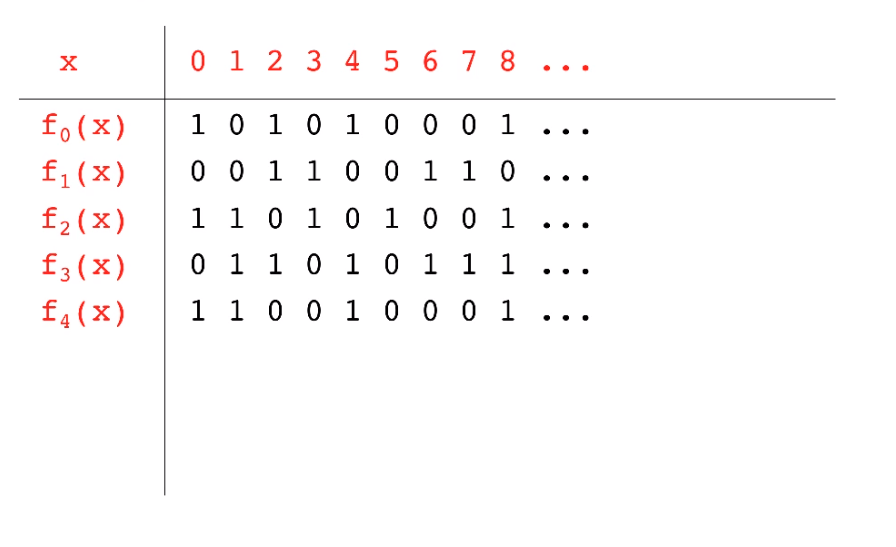
\includegraphics[scale=0.6]{3.png}
\end{center}
Definisco $g(x)$ 0 se $f_x(x) = 1$, 1 se $f_x(x) = 0$, $g$ non può corrispondere a nessuna delle $f_i$ della tabella, perché differisce da tutte le funzioni almeno nella diagonale principale.\\
$g(x)\:|\:0\:1\:1\:1\ldots$\\
Per assurdo $\exists\:j\:|\:g(x) = f_j(x)$ allora $g(j) = f_j(j)$ ma per la definizione è il suo complemento, quindi $g(j) \neq f_j(j)$ contraddizione.\\
Per qualunque numerazione scelta esiste sempre almeno una funzione esclusa, quindi $F$ non è numerabile.
\subsection{Algoritmi}
Qualunque modello si scelga, gli algoritmi devono essere descritti da sequenze finite di caratteri di un alfabeto finito $\Rightarrow$ sono possibilmente infiniti ma numerabili
%TODO problema dell'arresto
%TODO tesi C-T
\end{document}
